% !TEX root = ../Abschlussbericht_Schimmeliger_Keller.tex
%%
%%  Hochschule für Technik und Wirtschaft Berlin --  Projektabschlussbericht
%%
%% Kapitel 4 - Praktische Umsetzung
%%
%%

\chapter{Praktische Umsetzung} \label{Praktische Umsetzung}
\section{Verwendete Hardware} \label{Hardware}
\subsection{LoPy4-Development-Board} \label{LoPy4}

Das LoPy4 ist ein von Pycom Ltd. hergestelltes Development-Board für die Anwendungen im IoT-Bereich. Es unterstützt viele Schnittstellen und Übertragungsprotokolle, die für IoT-Anwendung von großer Relevanz sind. Die Abbildung \ref{fig:lopy-blockschaltbild} stellt die Funktionalitäten des LoPy4-Development-Boards in Form eines Blockdiagrammes  dar. 

\begin{figure}[h]
 \centering
 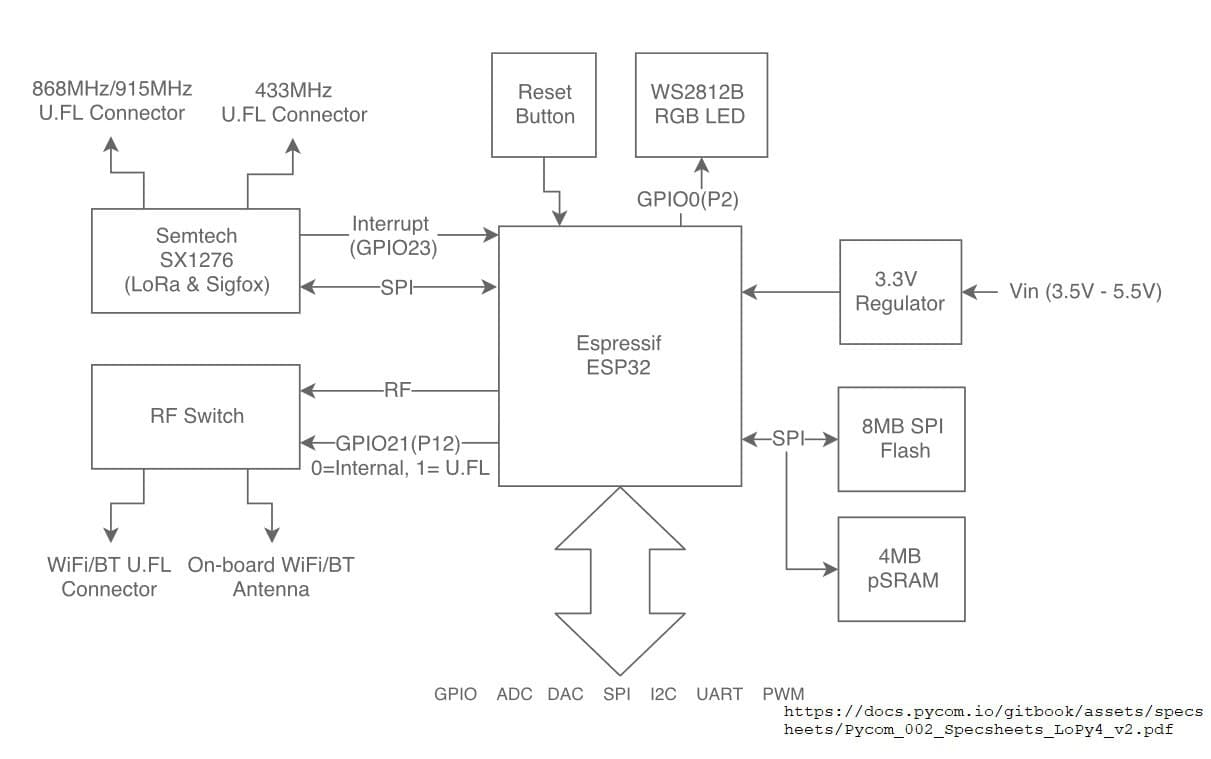
\includegraphics[width=1\textwidth]{pictures/blockdiagram_lopy}
 \caption[LoPy4-Blockdiagramm]{LoPy4-Blockdiagramm}\cite{Lopy2022}
 \label{fig:systemkonzept}
\end{figure}

Im Kern befindet sich ein Espressif ESP32 mit Xtensa dual-core-32-bit LX6 Mikroprozessor. Als Speicher verwendet es 520KB + 4MB RAM und einen externen 8MB Flash-Speicher, wohin auch der Code dann geladen wird. 
Zur Ein-/Ausgabe und der Steuerung von Sensoren und Aktoren, bietet das Board vielseitige Peripherien wie GPIO, ADC, DAC, SPI, I2C, UART und PWM an. 

Darüberhinaus verfügt das Entwicklungsboard über WLAN (802.11b/g/n/e/i), Bluetooth/Bluetooth Low Energy (BLE) v4.2, sowie LoRa und Sigfox Protokolle.  
Es lässt sich leicht mit einem Breadboard benutzen, um damit einfache Schaltungen, ohne zu löten, testen zu können. 

Für die WLAN und Bluetooth Anwendung kann man entweder die interne, im Board eingebaute, oder eine externe Antenne verwenden. Bei der Nutzung von LoRa und Sigfox muss man jedoch darauf achten, dass man unbedingt eine externe Antenne verwendet, denn sonst könnte damit der LoRa-Chip beschädigt und unbrauchbar gemacht werden. Dafür gibt es zwei Anschlussmöglichkeiten; einmal für das 868 MHz und einmal für das 433 MHz Frequenzband. 

Dafür wird der SX1276 LoRa-Transceiver-Chip der Firma Semtech verwendet.

\subsection{Mögliche Schaltung zum Selbstbauen} \label{LoPy4}

\subsection{DHT Sensormodul} \label{DHT}

Bei dem verwendeten Sensor handelt es sich um einen sog. DHT Sensor. Diesen gibt es in zwei verschiedenen Ausführungen, DHT11 und DHT22, wobei sich diese im auswertbaren Messbereich, der Messgenauigkeit und im Preis unterscheiden.

\begin{adjustwidth}{-1in}{-1in}% adjust the L and R margins by -1 inch
	\begin{center}
	
	        \begin{tabular}{ccc}
			\toprule
			 & \textbf{DHT11} & \textbf{DHT22}\\

			\midrule
			Betriebsspannung & \multicolumn{2}{c}{3 \dots 5 V DC}\\
			Stromverbrauch & \multicolumn{2}{c}{max. 2,5 mA während der Konvertierung}\\
			Temperaturbereich & -20\dots 60 °C & -40\dots 80 °C  \\
			Temperatur Genauigkeit & ± 2,0 °C & ± 0,5 °C\\
			Feuchtigkeit Messbereich & 20\%\dots90\% RH & 0\%\dots99,9\% RH\\
			Feuchtigkeit Genauigkeit & ± 5,0\% RH & ± 2\dots5\%\\
			Abtastrate & 1 Hz & 0,5 Hz \\

			\midrule
			Preis (bei reichelt elektronik) & 1,80 € & 6,80 €\\

			\bottomrule
	
	        \end{tabular}
		\label{}
		\captionof{table}{Vergleich DHT11 zu DHT22} \label{tab:vergleichDHT} 
	\end{center}
\end{adjustwidth}

Anzumerken ist noch, dass der DHT22 Sensorungefähr das doppelte Volumen des DHT11 Sensors hat. Interessant ist auch, dass der DHT11 Sensor ungefähr doppelt so häufig angesprochen werden kann, was vermutlich auf seiner weniger komplexen Schaltung beruht.\\
Für die meisten Anwendungsfälle würde wahrscheinlich ein DHT11 Sensor (oder mehrere parallel geschaltete DHT11 Sensoren) ausreichen, um ein weitgehend zuverlässiges Ergebnis zu erhalten.

\subsubsection{Kommunikation mit dem DHT Sensor\cite{dht}} 

Die Kommunikation mit dem DHT Sensor erfolgt über eine einzelne Leitung, was zum einen die Kosten reduziert, zum anderen aber auch die Reichweite der störungfreien Übertragung erhöht. Um den Sensor anzusprechen und die Daten anschließend auszulesen, muss der Datenstrom kodiert werden. Dies geschieht über ein Protokoll, welches die Kommunikation in drei Schritte aufteilt:
\begin{itemize} 
	\item Request (die Anfrage)
	\item Repsonse (die Antwort des Sensors)
	\item Data (die vom Sensor übertragenen Daten)
\end{itemize}


\begin{center}
	\begin{figure}[h]
	 
	 \noindent\makebox[\textwidth]{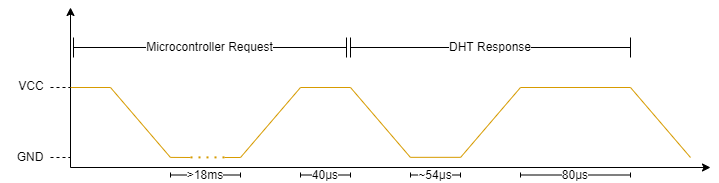
\includegraphics[width=1.1\textwidth]{pictures/dht_kommunikation1}}
	 \caption[DHT Kommunikation]{DHT Kommunikation}
	 \label{fig:dhtkommunikation}
	\end{figure}
\end{center}


Um den DHT Sensor dazu zu bringen, Messewerte zu senden, zieht der Microcontroller den Datenbus für mindestens 18ms auf Masse, um ihn anschließend für 40µs wieder auf Versorgungsspannungsniveau zu ziehen. Dadurch versteht der DHT Sensor, dass er beginnen soll Messwerte zu sammeln.\\
Der DHT Sensor antwortet zunächst mit einer Sequenz, bestehend aus einem ca. 54µs langen LOW und anschließend 80µs HIGH. 

\newpage

Nachfolgend sendet der DHT Sensor fünf Datenpakete, bestehend aus jeweils 8 Bit, welche die einzelnen Sensor Messwerte mit einer Prüfsumme darstellen. Insgesammt sendet der DHT Sensor somit 40 Bit.

\begin{center}
	\begin{figure}[h]
	 
	 \noindent\makebox[\textwidth]{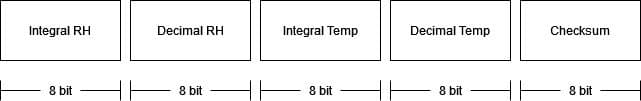
\includegraphics[width=0.9\textwidth]{pictures/dht11_dataframe}}
	 \caption[DHT Paketstruktur]{DHT Paketstruktur}
	 \label{fig:dhtpaketstruktur}
	\end{figure}
\end{center}

Die einzelnen Sensor Messwerte sind noch in Integral Anteil und Dezimal Anteil unterteilt, wobei die einzelnen Bits sich durch die dauer des HIGH Signals nach einem 54µs langem LOW Singal unterscheiden.

\begin{center}
	\begin{figure}[h]
	 
	 \noindent\makebox[\textwidth]{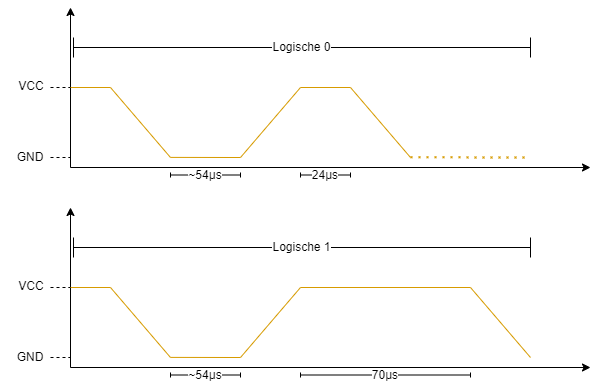
\includegraphics[width=0.9\textwidth]{pictures/dht_kommunikation2}}
	 \caption[DHT Bit Identifikation]{DHT Bit Identifikation}
	 \label{fig:dhtbits}
	\end{figure}
\end{center}

Abschließend sendet der DHT Sensor ein ca. 54µs langes LOW Signal, wonach der Bus wieder auf Versorgungsspannungsniveau gezogen wird und der Sensor in den Idle Mode geht.



\newpage

\subsection{Restliche Hardware} \label{Restliche Hardware}


\begin{itemize} 
	\item \textbf{Antenne:}  Bei der verwendeten Antenne handelt es sich um eine Multiband Antenne, welche für mehrere Freuquenzbänder (unter anderem das LoRa Freuquenzband) genutz werden kann.
	\item \textbf{USB Kabel:} Wir verwenden ein Daten-USB Kabel welches besonders geschirmt ist und eine maximal Länge von ca. 10cm aufweist. Wir hatten teilweise Probleme mit anderen USB Kabeln.
\end{itemize}



\section{Beschreibung der Software} \label{Software}

Für unser Projekt haben wir drei verschiedene, miteinander interagierende Software Komponenten realisiert, welche über eine Schnittstelle (Interface) miteinander kommunizieren. 
Der Vorteil einer solchen Architektur ist, dass die einzelnen Komponenten sich unter umständen wiederverwenden lassen und sich im Idealfall so eine Software modular aufbauen lässt.
Da wir als Programmiersprache ausschließlich Python bzw. Micropython verwendet haben, könnte man argumentieren, dass unsere Software automatisch Modular ist, da sich in der Theorie alle programmierten Komponenten in Python wiederverwenden lassen.
Dies ist aber sehr verallgemeinert gesprochen, da gerade die Programmierung der Mikrocontroller definitiv auch Individualsoftware benötigt, welche sich aber immerhin nicht nur auf einer einzelnen Mikrocontrollerfamilie ausführen funktionieren würde.
Anzumerken ist noch, dass für unsere finale Version des Projektes vermutlich nur eine einzelne Softwarekomponente notwendig wäre.\\
Für die Programmierung der Mikrocontroller verwenden wir die Programmiersprache Micropython, welche eine schlanke und schnelle Implementation der Programmiersprache Python ist, welche für Mikrocontroller optimiert wurde.

\newpage


\subsection{1. Komponente: Sensoransteuerung und der Versand der Daten mittels LoRa(WAN)} \label{Sender}


\begin{center}
	\begin{figure}[h]
	 
	 \noindent\makebox[\textwidth]{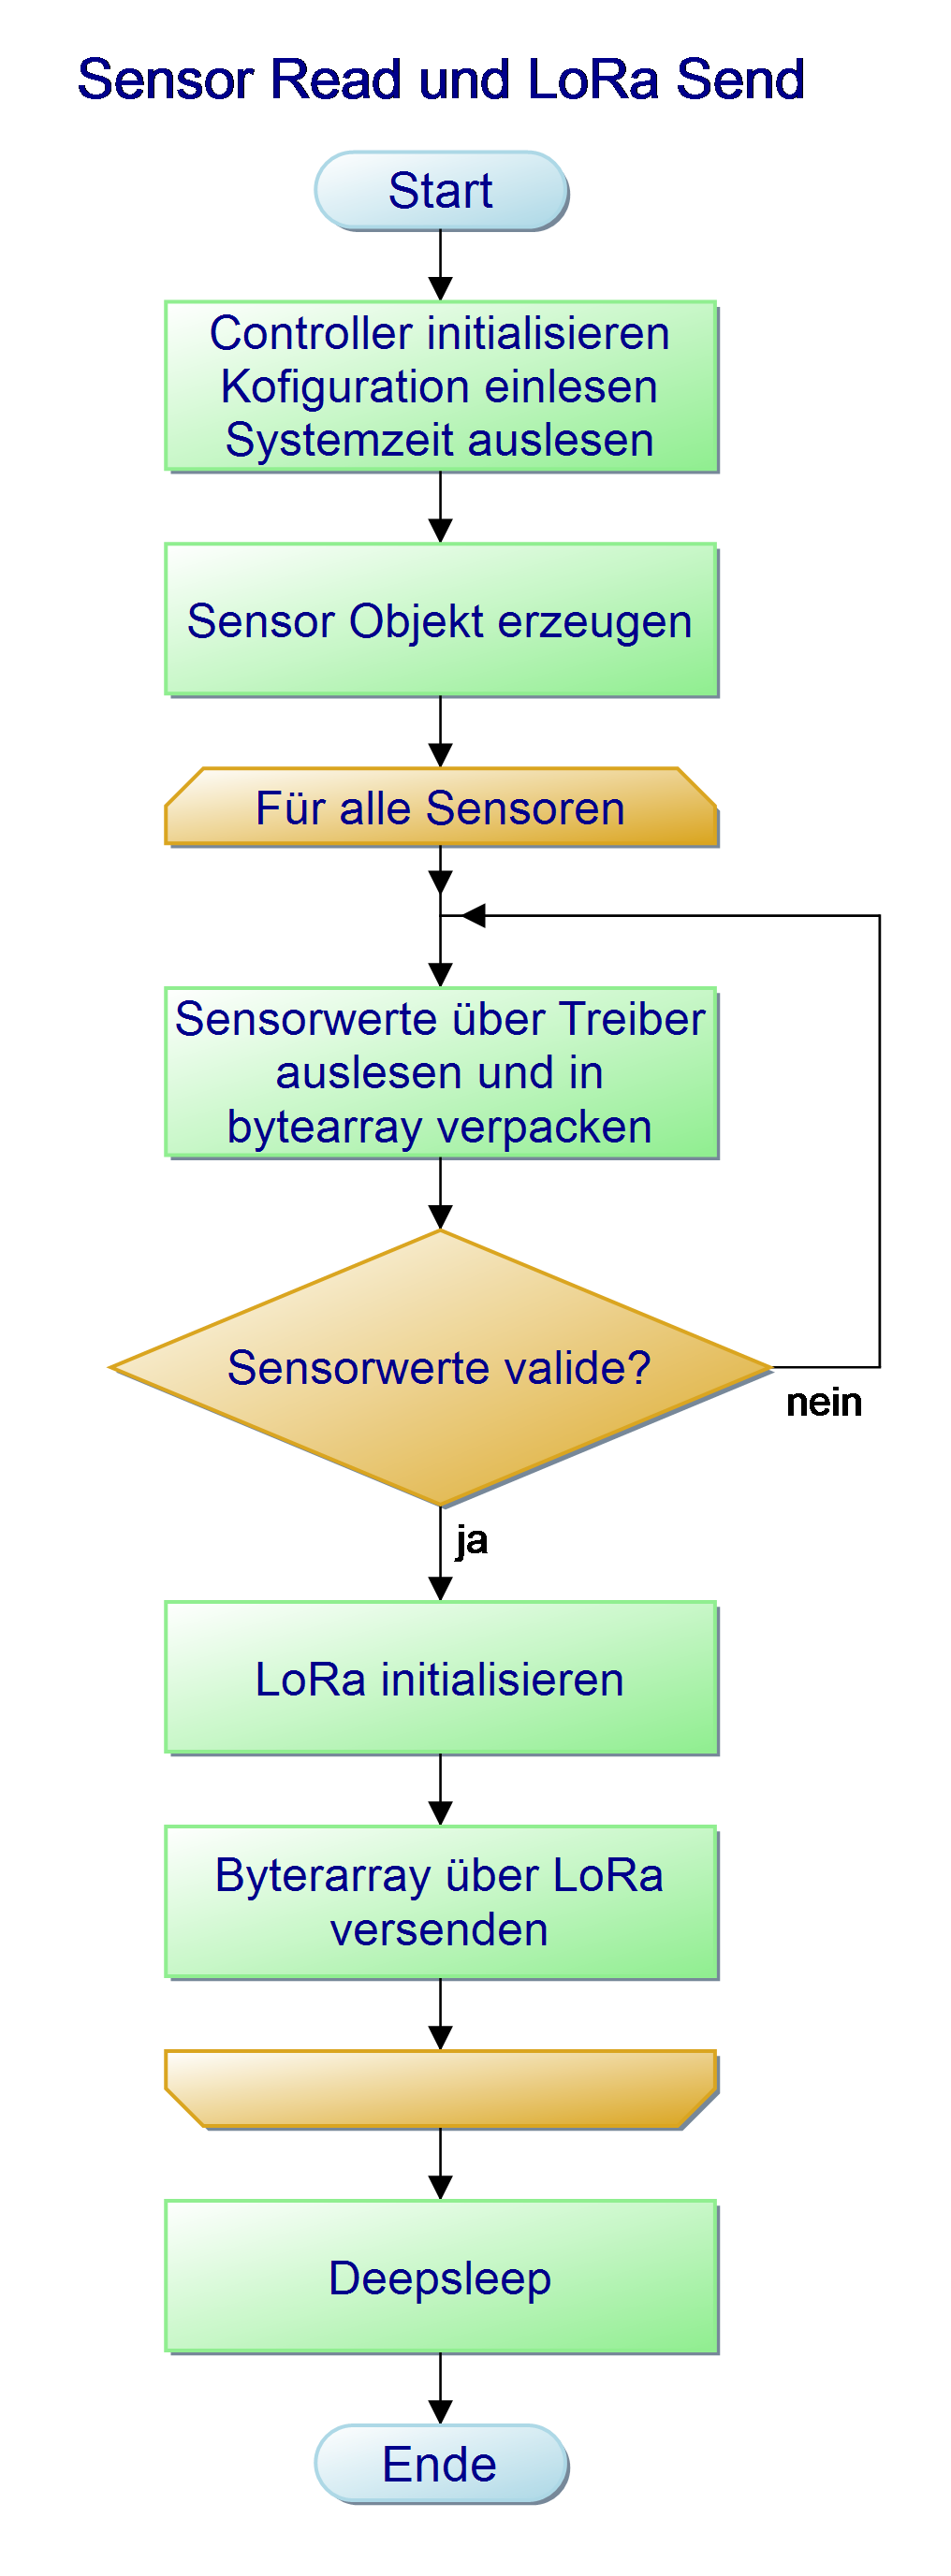
\includegraphics[width=0.35\textwidth]{pictures/sens_read_lora_send}}
	 \caption[PAP komponente 1]{Programm Ablauf: Komponente 1}
	 \label{fig:lorasendsensorread}
	\end{figure}
\end{center}

Zunächst wird der Microcontroller initialisiert, wobei er standartmäßig mit allen Modulen (WiFi, LoRa, etc.) im aktivierten Zustand startet. Dieser Umstand beruht darauf, dass wir die PyCom Plattform nutzen, welche wenig vorab Konfiguration ermöglicht.\\
Jegliche Konfigurationsmöglichkeiten unserer Programme haben wir in extern Dateien im JSON Format abgelegt, welche im nächsten Schritt eingelesen werden. In der Konfigurationsdatei können unter Anderem die Dauer, die der Microcontroller im Schlafmodus verbringen soll, sowie die einzelnen Sensoren definiert werden.\\
Um das anbinden mehrere Sensonren zu ermöglichen haben wir uns dazu entschieden, eine Klasse zu programmieren, welche eben dieses Sensorobjekt darstellen soll. Der Treiber wurde von einem Benutzer auf github veröffentlicht, funktioniert aber im Prinzip nach dem oben genannten Verfahren, was bedeutet, dass zunächst eine gewisse Zeit gewartet wird, anschließend das Bus auf GND Niveau gezogen wird, um den Sensor mitzuteilen, dass er doch bitte anfängt Messwerte zu sammeln. Nachdem der Sensor eine Antwort gegeben hat, werden die empfangenen Bits zunächst alle gesammelt und anschließend in 5 einzelne Bytepakete decodiert. Abschließend prüft der Treiber mithilfer der Prüfsumme, ob die empfangenen Daten Sinn machen.\\ Je nach Sensortyp (DHT11/22) werden die empfangenen Daten nochmals in den richtigen Wertebereich \grqq verschoben\grqq.\\
Anschließend werden für alle initialisierten Sensoren, über den Treiber die aktuellen Messwerte eingelesen und in ein bytearray verpackt, wobei hier schon das erste mal geschaut wird, ob die gemessen Sensorwerte überhaupt Sinn ergeben bzw. in dem vom Hersteller angebenen Bereich fallen, da es selbst bei der korrekten Dekodierung immernoch zu unsinnigen Werten kommen kann. 
Wurde dieser Test erfolgreich bestanden wird im Microcontroller über das LoRa Modul über eine Bibliothek initialisiert und die ermittelten Werte werden versendet.\\ Ein weiterer Bestandteil des bytearrays ist die aktuelle Systemzeit, welche verwendet wird, um im späteren Verlauf ermitteln zu können, ob es sich wirklich um ein neues empfangenes Datenpaket handelt, oder ob das Paket in irgendeinem Puffer zunächst verloren gegangen ist und zufällig wieder ins Tageslicht gerückt ist.\\
Zu guter Letzt wird der Microcontroller in den Schlafmodus versetzt, wobei die Zeit, die er im stromsparenden Modus verbringt benutzerdefiniert ist. Die Systemzeit läuft auch im Schlafmodus weiter, solange der Microcontroller mit Strom versorgt wird, nur das LoRa-Modul muss neu initialisiert werden.\\

\newpage

\subsection{2. Komponente: Emfangen der Daten und Versand ins Internet} \label{Empfänger}

\begin{center}
	\begin{figure}[h]
	 
	 \noindent\makebox[\textwidth]{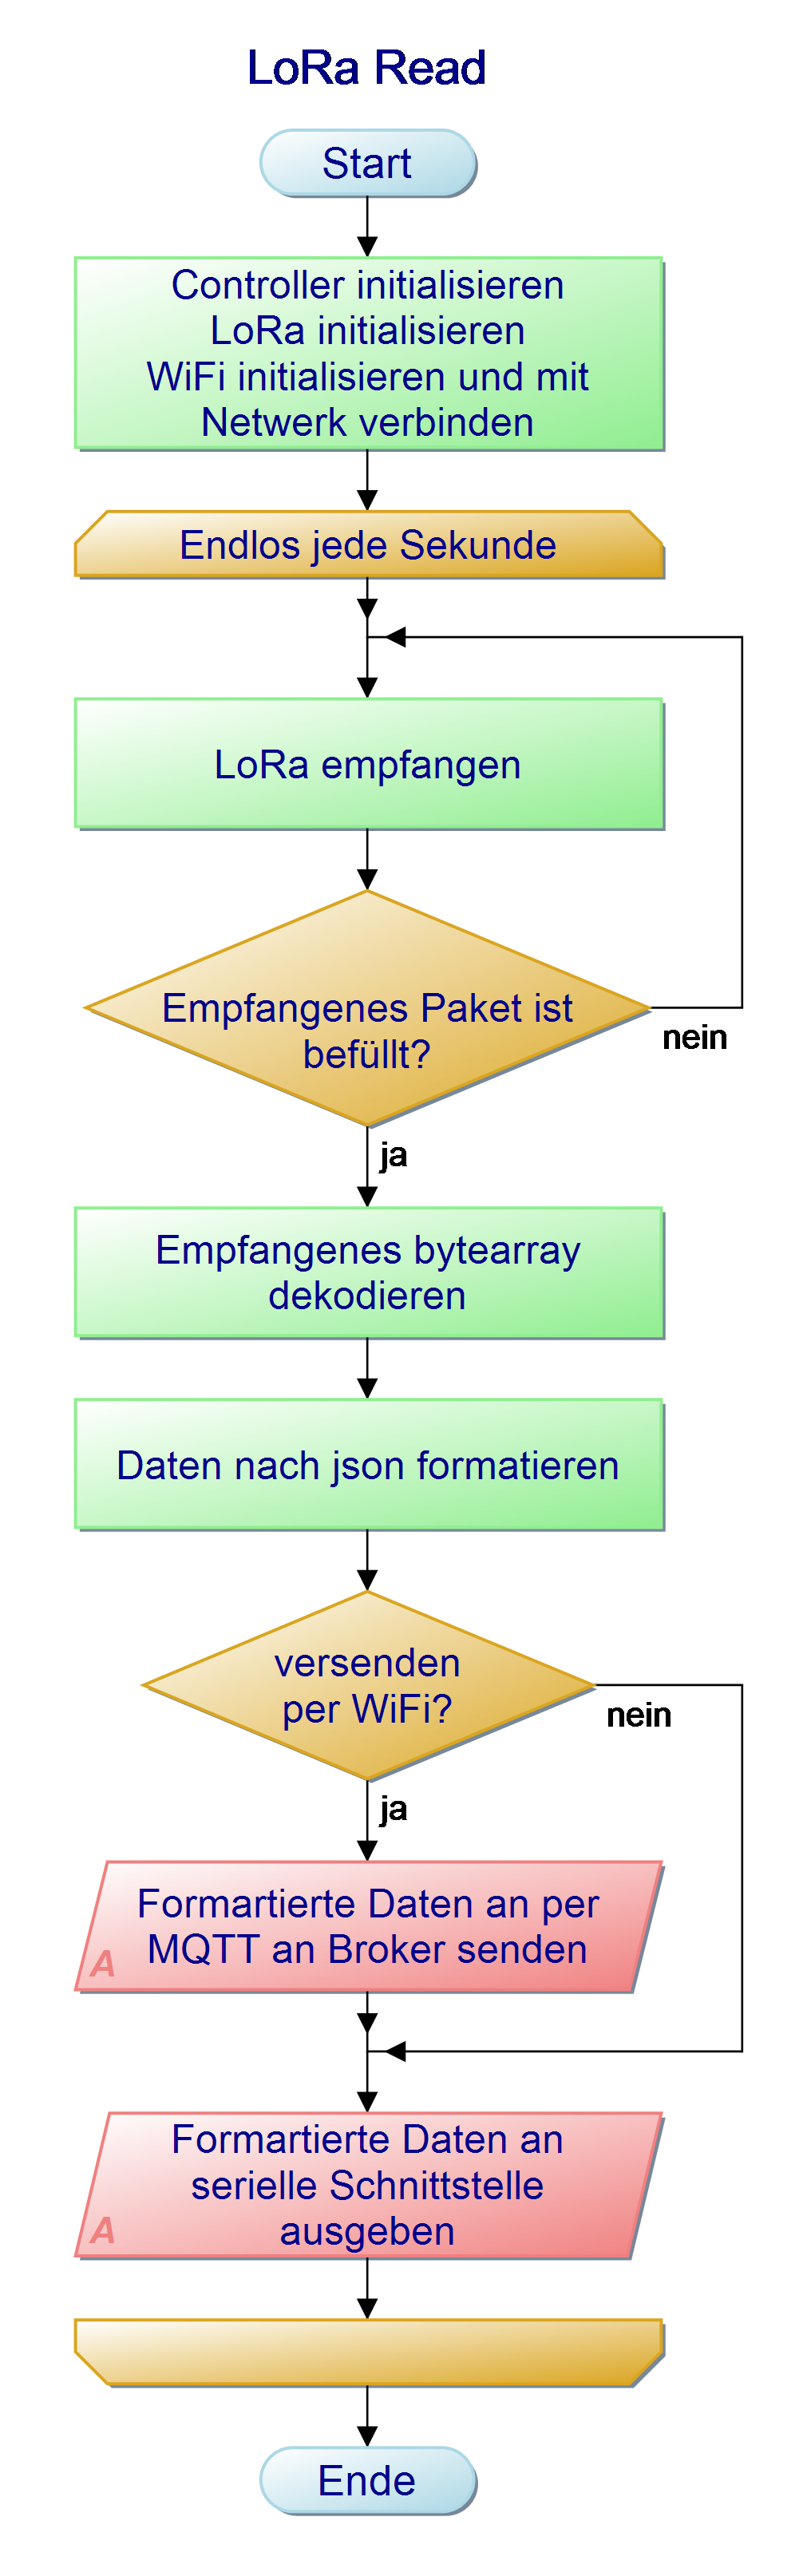
\includegraphics[width=0.3\textwidth]{pictures/LoRaRead}}
	 \caption[PAP komponente 2]{Programm Ablauf: Komponente 2}
	 \label{fig:lorareadwifisend}
	\end{figure}
\end{center}

Diese Softwarekomponente läuft schlussendlich auf dem LoRa Gateway, bzw. in unserem Fall dem zweiten Microcontroller, welcher in unserem Fall den Empfänger bei der P2P Verbindung darstellt.
Wie bei der ersten Komponente, wird zunächst der Microcontroller initialisiert. Des Weiteren werden Konfigurationsdaten eingelesen, welche für die optionale WiFi Verbindung und das senden an die MQTT Broker benötigt werden. Möchte man die Sensordaten einfach nur über eine serielle Schnittstelle auslesen, können diese Felder entsprechend leer gelassen werden.
Außerdem wird in dieser Komponente das LoRa Modul direkt initialisiert, da dies nur einmalig geschehen muss.\\
Es beginnt eine Endlosschleife

\newpage

\subsection{3. Komponente: Manuelles abrufen und versenden der veröffentlichten Daten} \label{PubSub}

\begin{center}
	\begin{figure}[h]
	 
	 \noindent\makebox[\textwidth]{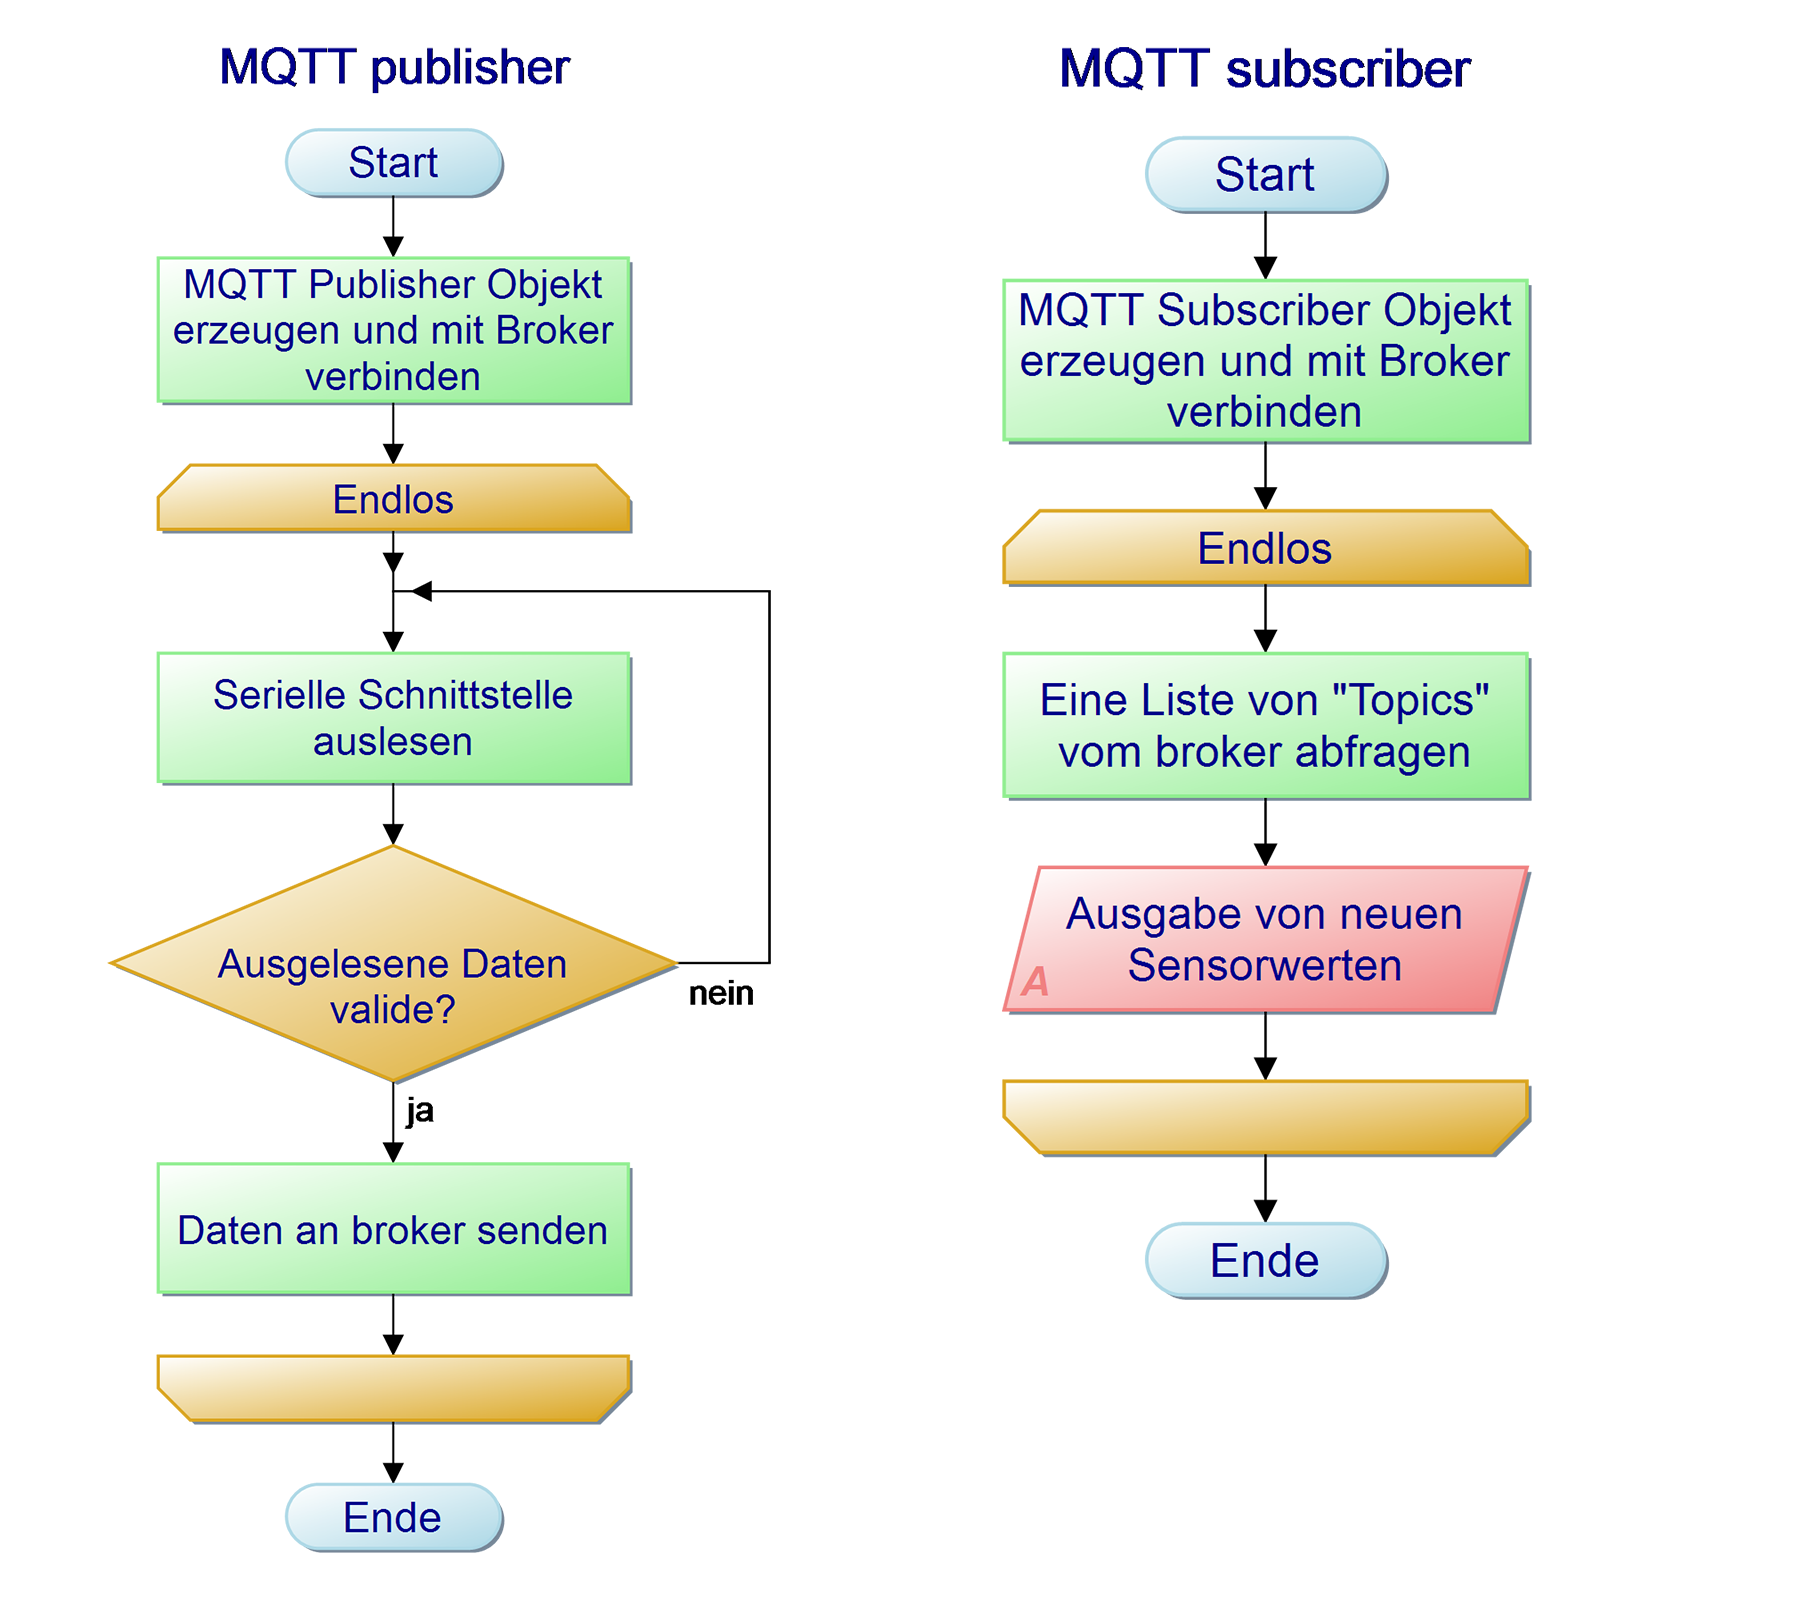
\includegraphics[width=0.9\textwidth]{pictures/MQTTpubsub}}
	 \caption[PAP komponente 3]{Programm Ablauf: Komponente 3}
	 \label{fig:MQTTpubsub}
	\end{figure}
\end{center}

abc

\newpage

\section{Visualisierung der Sensordaten} \label{Dashboard und Visualisierung}

abc

\newpage


\section{Berechnung der Laufzeit im Batteriebetrieb} \label{Simulation}

\begin{center}
	\begin{figure}[h]
	 
	 \noindent\makebox[\textwidth]{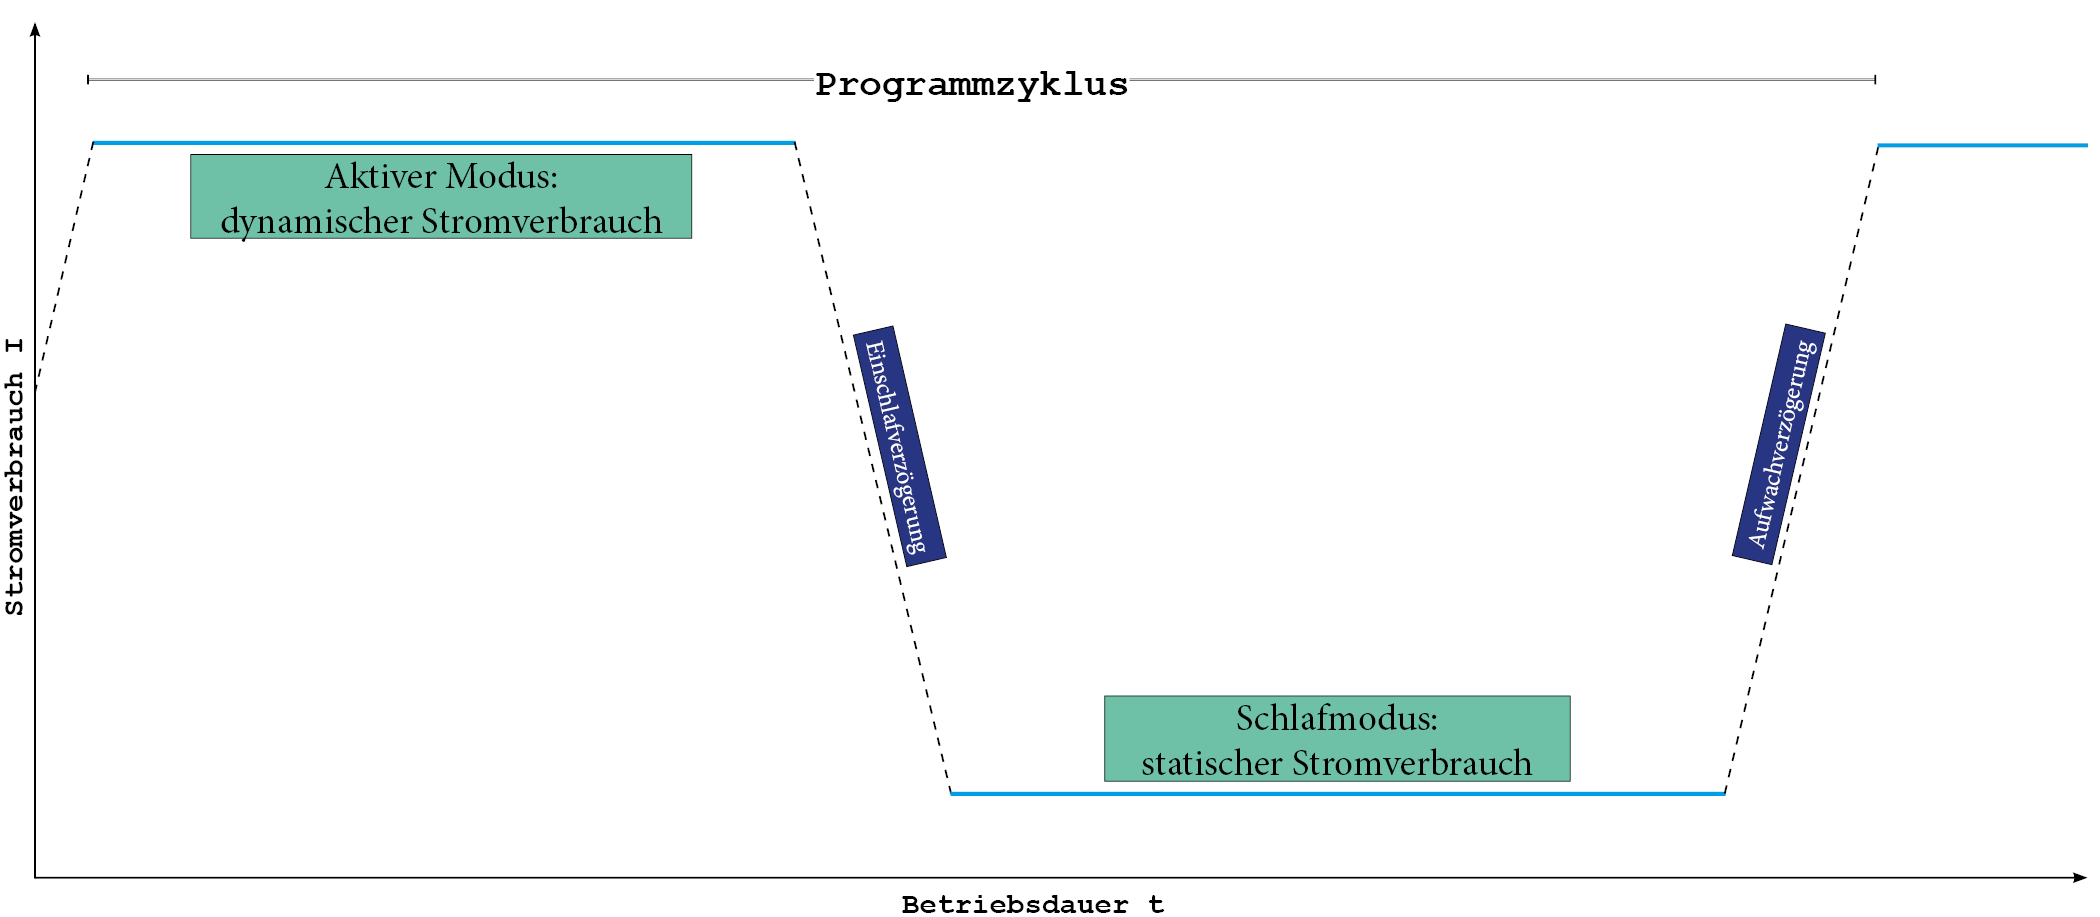
\includegraphics[width=1.1\textwidth]{pictures/programmzyklus}}
	 \caption[Stromverbrauch während eines Programmzyklus]{Stromverbrauch während eines Programmzyklus}
	 \label{fig:stromzyklus}
	\end{figure}
\end{center}

abc

\newpage
